\documentclass[a4paper, 12pt]{article}
\usepackage{tikz}
\usetikzlibrary{shapes,arrows}
\usetikzlibrary{shapes.geometric}
\usepackage{fullpage}
\usepackage{cite}
\usepackage{hyperref}
\usepackage{amsmath}
\usepackage{amsthm}
\usepackage{amssymb}

\author{Ryan Kinnear - 200273748 \\ Raza Rauf}
\title{Implementation of Software Defined Radio}
\date{\today}

\newtheorem{thm:NSST}{Nyquist-Shannon Sampling Theorem}

\begin{document}

\maketitle

\newpage
\tableofcontents
\newpage
\listoffigures
\newpage

\section{Introduction}
\label{sec:intro}
Modern wireless systems are a ubiquitous part of society.  There billions of people accessing the internet, many of them wirelessly.  This includes through home, office, or public WiFi networks, as well as through cellular networks.  The electromagnetic spectrum is also exploited for radio astronomy, Radio Frequency Identification (RFID), radar etc...  

In the past, all radio \footnote{The word \textit{radio} is used to refer to any device that makes use of the EM spectrum.  This does not refer only to communication systems, and certainly not only to radios made for receiving music} functionality was necessarily implemented in hardware using traditional electronics (transistors, capacitors, transformers...).  This also includes implementation with integrated circuits, even highly integrated devices with millions of transistors.  While the highly integrated ICs seem very modern, these radios offer no flexibility.  It is very costly to upgrade this type of radio equipment to take advantage of more modern protocols and algorithms - the entire device needs to be replaced.

The modern proliferation of high speed digital electronics, VLSI, and the mathematical understanding of digital signal processing has naturally lead to the integration of digital processing power and radio devices.  A radio that has some dynamic reconfigurability is referred to as a \textit{software controlled radio}.  This may be a radio capable of dynamically choosing between the size of a QAM constellation based on noise levels, tuning the weights of a digital equalizing filter, or dynamically varying transmit power levels.  However, the fundamental demodulator is fixed in hardware and cannot be modified.  So the problem of upgrading radio equipment to make use of newer protocols and algorithms still exists.

Software defined radio (SDR) is a solution to the problem of limited flexibility.  In SDR, the vast majority of the signal processing is implemented in reconfigurable hardware (FPGAs \cite{fpga_defn}) or in software running on either a Digital Signal Processor (DSP \cite{dsp_defn}) or a General Purpose Processor (GPP) such as the one in your computer.  These devices are very easy to reconfigure, and thus the cost of upgrading to newer protocols and algorithms is drastically reduced.  Not only that but these upgrades or bug fixes can be performed remotely with ease.  Moreover, the ease with which the system is reconfigured allows one to use SDR as a test bed for development.

A further advantage of SDR is that both analog systems and integrated circuits are \textit{extremely} hard to design.  For a mixed signal integrated circuit that is 90\% digital, and 10\% analog, the analog design will take 90\% of the design time \cite{ana_why}.  To design a new integrated circuit every time a new protocol needs to be implemented would be \textit{ridiculous}.

%Write about how the report proceeds.
%Overview of SDR
%Our implementation
%Design goals and strategies
%Testing
%Uses of SDR
%Cognitive Radio

\section{Fundamentals of SDR}
\label{sec:sdr_funadamentals}
\subsection{The Ideal SDR}
\label{sec:ideal_sdr}
An ideal SDR consists almost entirely of reconfigurable hardware, and digital signal processing. The ultimate goal is to acheive flexibility, and minimize the amount of analog design.  This ideal SDR would consist of an antenna, an analog to digital and digital to analog converter, a circulator, and a processor (see figure \ref{fig:ideal_sdr}).

%SDR architecture image
%------------------------------------------------------------------
%Damn this was hard to draw.

\tikzstyle{ADC} = [draw, fill=blue!20, text width=5em, 
    text centered, minimum height=2.5em]
\tikzstyle{DAC} = [draw, draw, fill=blue!20, text width=5em, 
    text centered, minimum height=2.5em]
\tikzstyle{Data} = [text width=5em, text centered, minimum height = 2.5em]
\tikzstyle{DSP} = [draw, text width=6em, fill=red!20, 
    minimum height=12em, rounded corners, text centered]
\tikzstyle{out} = [coordinate]
\tikzstyle{circulator} = [circle, draw, minimum height = 3em]
\tikzstyle{antenna} = [regular polygon, regular polygon sides = 3, thick, draw, fill=green!20, text width = 2em, shape border rotate = 180]

%\tikzstyle{antenna} = [draw]

\def\blockdist{2.3}
\def\edgedist{2.5}

\begin{figure}[ht]
\caption{Ideal SDR Architecture}
\label{fig:ideal_sdr}
\centering
\begin{tikzpicture}[auto, thick, node distance=2cm, >=latex']
  %The processor node goes right in the middle
  \node (processor) [DSP] {DSP / GPP};
  %Then place the ADC/DAC relative to the processor
  \path (processor.140)+(-\blockdist, 0) node (ADC) [ADC] {ADC};
  \path (processor.-140)+(-\blockdist, 0) node (DAC) [DAC] {DAC};
  %And draw arrows between them
  \draw [->] (ADC) -- (processor.west |- ADC);
  \draw [<-] (DAC) -- (processor.west |- DAC);
  
  %Place the circulator
  \path (processor)+(-3*\blockdist,0) node (circulator) [circulator] {CIRC};
  \draw [<-] (ADC.west) -- (circulator);
  \draw [->] (DAC.west) -- (circulator);

  \path (circulator)+(-1.2*\blockdist,0) node (antenna) [antenna] {ANT};
  \draw [<->] (antenna) -- (circulator.west);

  %Then place outputs relative to the processor
  \path (processor.150)+(2*\blockdist,0) node (out) [Data] {Data Out};
  \path (processor.-150)+(2*\blockdist,0) node (in) [Data] {Data In};
  %And arrows between them
  \draw [<-] (out) -- (processor.east |- out);
  \draw [->] (in) -- (processor.east |- in);

\end{tikzpicture}
\end{figure}
%------------------------------------------------------------------

This has the absolute minimum amount of analog components, and all of the signal processing is done in software.  While there is nothing wrong with this architecture in theory, it is obviously very difficult to implement in practice.  

Historically, the main problem was with the speed of the data converters.  However, there are now ADCs that can directly sample RF frequency signals \cite{gsps_adc}.  These ADCs are very sophisticated, and are far beyond the scope of this project, but high performance commercial software defined radios do make use of ultra high speed data converters.  For the rest of us, there is \textit{undersampling} (section \ref{sec:undersampling}).  This enables one to sample RF signals at rates far lower than twice the highest frequency component.

On the transmission side, it isn't possible to connect a DAC directly to an antenna.  There needs to be at least some analog components to provide power and filtering.

Another issue is the data rate.  A sample rate at 5GSPs might be able to effectively digitize an RF signal, but the torrent of data (40+ Gbps) is far beyond the capability of any GPP or DSP.  This is where FPGAs and \textit{downsampling} (section \ref{sec:downsampling}) come in.

\subsection{Undersampling}
\label{sec:undersampling}
The Nyquist-Shannon Sampling Theorem is the most important theorem in digital signal processing.

\begin{thm:NSST}
\label{thm:NSST}
  If a function $f(t)$ is bandlimited to B hertz \footnote{A function is bandlimited to B hertz if it's it's Fourier transform has compact support [$-B/2, B/2$]} then $f(t)$ can be completely reconstructed from discrete samples of $f(t)$ at intervals $\frac{1}{2B}$.
\end{thm:NSST}

If we let $T = \frac{1}{2B}$ be the sampling interval, The specific formula for reconstruction is given by the sinc interpolator:

\begin{equation}
\label{eq:sinc_interpolation}
f(t) = \Big[\sum_{n=-\infty}^{\infty}{f(nT)\delta(t - nT)\Big]}*sinc(\frac{\pi t}{T}) = \sum_{n=-\infty}^{\infty}{f(nT)sinc(\pi\frac{t - nT}{T})}
\end{equation}

A critical piece of this theorem that seems to be frequently misunderstood is that the signal must be \textit{bandlimited} to B hertz.  This does \textit{not} mean that the highest frequency component needs to be below B hertz.  If the highest frequency component of the signal is below B hertz, then the assumptions of the theorem still hold.  It is a sufficient condition, however it is \textit{not necessary}.

If the signal is bandlimited to B hertz, but has spectral components greater than B (that is, is it a bandpass signal, see figure \ref{fig:bandpass_signal}), it is still possible to sample the signal without losing any information.  However, the effects of \textit{aliasing} will still be present.  But, aliasing is really not a big problem, as will be seen shortly.

\begin{figure}[ht]
\caption{A bandpass signal limited to B hertz}
\label{fig:bandpass_signal}
\centering
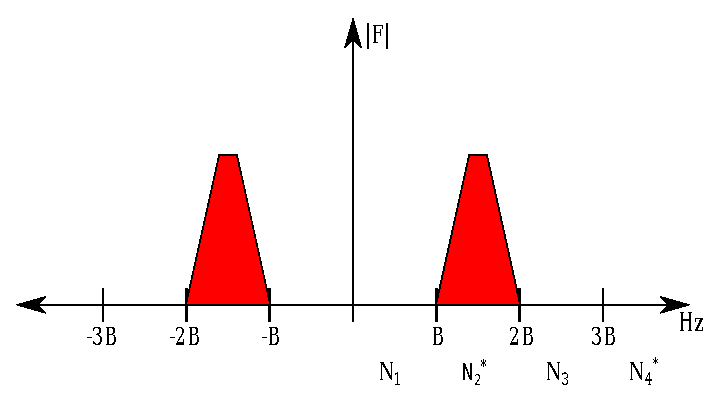
\includegraphics[width=11cm]{images/bandpass_signal.eps}
\end{figure}

The effect of sampling is to break up the frequency spectrum into ranges of width B.  That is, the frequency axis is partitioned into sets of the form $[nB, (n+1)B], n \in \mathbb{Z}$.  Each of these sets is referred to as a \textit{Nyquist Zone}.  They are labeled $N_1, N_2, ...$ in figure \ref{fig:bandpass_signal}.  Note that $N_1$ is the baseband.  Each of these zones will \textit{alias} or \textit{fold} back to baseband ($N_1$).  The best way to visualize this is to imagine folding the right half plane vertically at each $B, 2B, 3B ...$.  See figure \ref{fig:bandpass_sampling}.  Notice that the even nyquist zones get mirrored about the $B/2$ axis.

\begin{figure}[ht]
\caption{The effect of sampling}
\label{fig:bandpass_sampling}
\centering
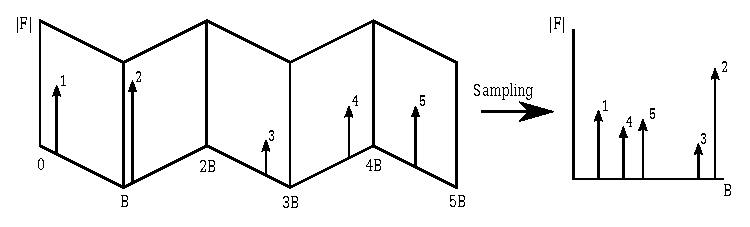
\includegraphics[width=13cm]{images/bandpass_sampling.eps}
\end{figure}

It should now be clear that analog to digital converters can be used to effectively digitize signals, even if they are at a very high frequency.  The only requirement is on the \textit{bandwidth} of the signal.  Naturally, a bandpass filter is needed to cut out the out of band signals.  In undersampling a bandpass filter is used for anti-aliasing, it seems to be commonly assumed that lowpass filters are always used for anti-aliasing.  This is only the case when sampling a signal that falls entirely in $N_1$.

There is another question to be looked at here, which is how to actually choose the sample rate?  If the spectrum of the signal you wish to digitize doesn't conveniently fall into one of the Nyquist zones, then some of the spectrum will be mirrored, and the other part won't be.  This will lead to a loss of information.  Also, it is convenient to ensure that the signal falls into an odd Nyquist zone, so that it doesn't get mirrored.  The criteria for the sampling rate can then be easily written down mathematically, where $f_c$ is the center frequency.

\begin{equation}
\label{eq:sample_rate}
\begin{aligned}
  &f_s > 2B \\
  &f_c - \frac{1}{2}B > nf_s \\
  &f_c + \frac{1}{2}B < \frac{1}{2}(2n + 1)f_s \\
\end{aligned}
\end{equation}

If for a given sample rate $f_s$, $\exists n \in \mathbb{N}$ satisfying the equations in (\ref{eq:sample_rate}) then that sample rate can be used to bandpass sample the signal.  Moreover, $n+1$ gives the nyquist zone the signal falls into.

\subsection{Downsampling}
\label{sec:downsampling}

%A software defined radio (SDR) is essentially a digital radio.  An analog front end device such as a DVB-T USB dongle \cite{usb_dongle}, HackRF \cite{hackrf}, or the USRP \cite{usrp} receives and digitizes a radio frequency signal and sends the samples to a computer.  The ideal software defined radio consists of an analog to digital convert with one end connected directly to an antenna, and the other end connected to a computer.  A realistic implementation requires a significant analog component to digitize RF signals, as well as significant preprocessing on the digital signal (usually accomplished by an FPGA or DSP).

\section{}

\clearpage
\bibliography{../refs/fourth_year.bib}
\bibliographystyle{IEEEtran}

\end{document}
